\subsection{Mechanizmy Kubernetes stojące za Lupus}
Niniejsza praca zakłada znajomość czytelnika platformy Kubernetes na podstawowym poziomie.

\subsubsection{Kontroler}
Działanie Kubernetes opiera się na zamkniętej pętli sterowania [odnośnik do artykułu]. \textbf{Aktualny Stan} systemu zapisany jest w bazie etcd. \textbf{Stan Pożądany} wyrażony jest poprzez pliki manifestacyjne. Każdy \textit{Obiekt API} posiada swoją sekcję $`spec`$, to ona definiuje pożądany stan danego obiektu. Każdy obiekt ma swój kontroler, który rekoncyliuję aktualny stan do stan pożądanego. Kontroler jest to proces działający w warstwie sterowania Kubernetes. Każdy typ (ang. \textit{Kind}) wbudowanych zasobów (ang. \textit{buil-in resources}) ma swój kontroler stworzony przez zespół Kubernetes. Kontrolery każdego typu zasobu działają w podzie \texttt{kube-controller-manager}. 

\begin{figure}[!h]
    \centering 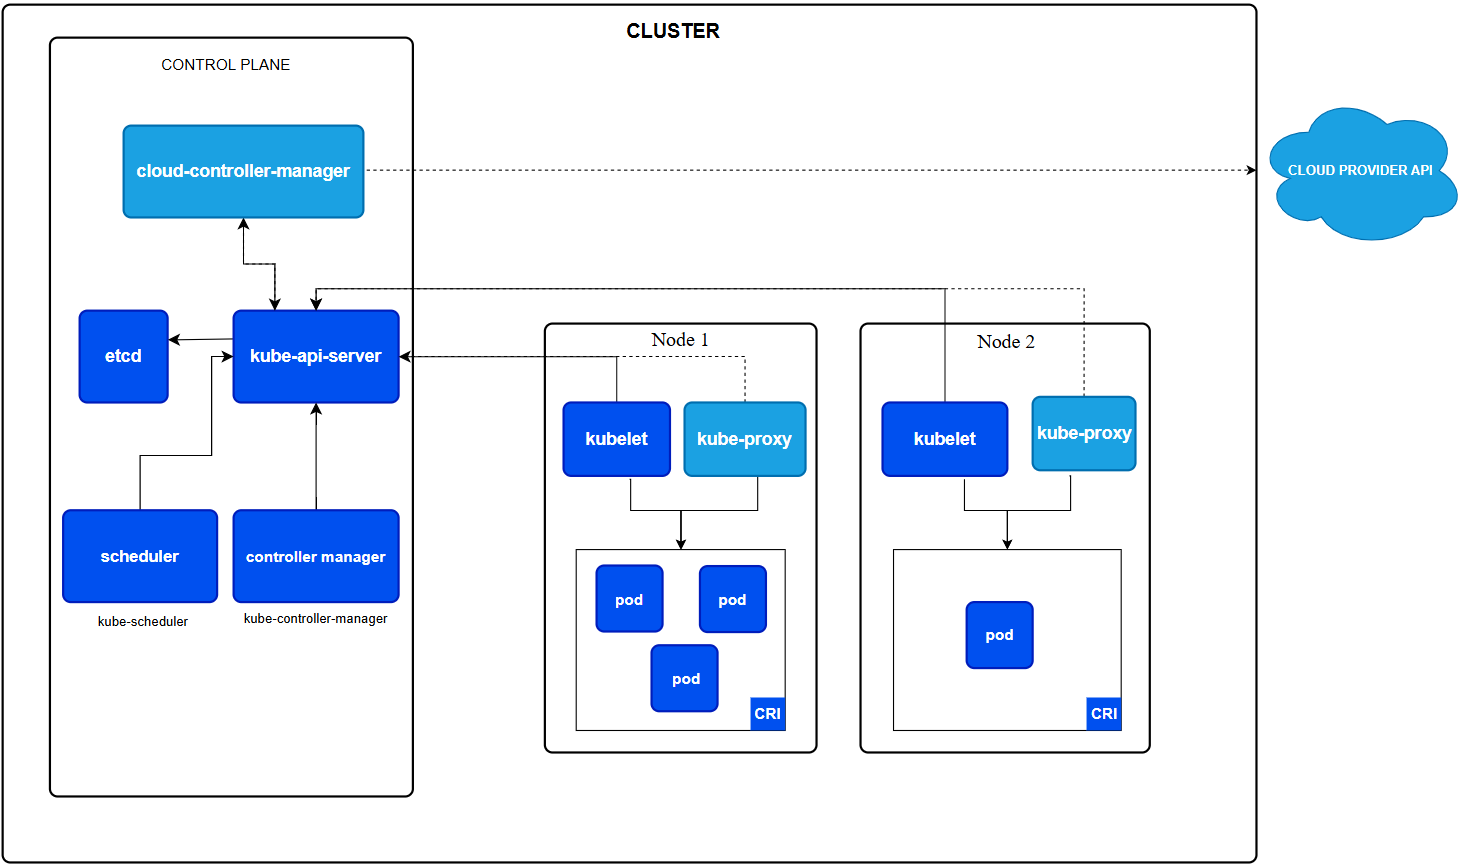
\includegraphics[width=1\linewidth]{42-k8s-arch.png}
    \caption{Architektura Kubernetes. Źródło: \url{https://kubernetes.io/docs/concepts/architecture/}}\label{fig:42-k8s-arch}
\end{figure}

Flow pracy kontrolera pokazano na rysunku \ref{fig:42-flow}. Gdy `kube-api-server' otrzyma żądanie zmiany danego obiektu API zanim `kube-api-server` zleci utrwalenie tych zmian wykona tzw. \textit{webhooki} do kontrolera danego obiektu. Webhooki nie są jednakże istotne z punktu widzenia niniejszej pracy dyplomowej \footnote{Dla zainteresowanych tematem: link}. Następnie, gdy doszło do zmian w obiekcie, kontroler zostaje o tym poinformowany. Jego misją jest rekoncyliacja, czyli porównanie aktualnego stanu obiektu ze stanem pożądanym. Kontroler zawiera w sobie logikę rekoncyliacji, która przybliży oba stany do siebie. Wykonanie logiki wiążę się często z przeprowadzeniem różnych akcji przez kontroler w innych częściach klastra. 

\begin{figure}[!h]
    \centering 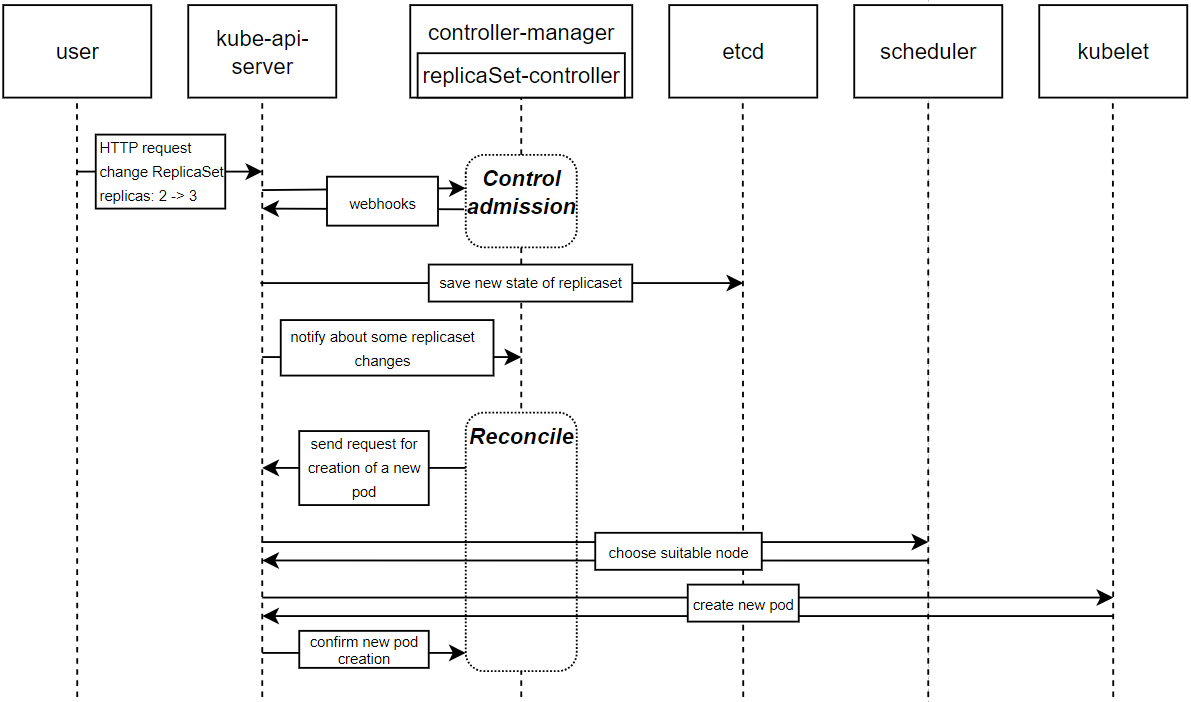
\includegraphics[width=1\linewidth]{42-flow.png}
    \caption{Flow pracy kontrolera. Źródło: Opracowanie własne.}\label{fig:42-flow}
\end{figure}

\subsubsection{Zasoby własne} 

\hyperlink{def:zasoby-wlasne}{\textit{Zasoby własne} (ang. \textit{Custom Resources})} rozszerzają wbudowane zasoby (ang. \textit{buit-in resources}) o niestandardowe, zdefiniowane przez użytkownika. Najczęściej tworzone są w celu zarządzania konfiguracją skomplikowanych lub stanowych aplikacji. 

Czasami wbudowane typy zasobów (jak Pody, Wdrożenia (ang. \textit{Deployments}), Serwisy (ang. \textit{Services})) nie są dla nas wystarczające, dlatego Kubernetes udostępnia możliwość rejestrowania nowych typów. Aby tego dokonać należy stworzyć plik manifestacyjny YAML typu \textit{Custom Resource Definition} a następnie zaaplikować go w klastrze. Po pomyślnej operacji, będzie można tworzyć obiekty nowego typu.

\subsubsection{Operatory}

Mechanizm ten służy do rozszerzania możliwości Kubernetes. Kiedy tworzymy Zasoby Własne (ang. \textit{Custom Resources}), możemy również implementować dla nich kontrolery. Takie podejście nazywane jest "wzorem operatora" ("operator-pattern"). Często takie kontrolery nazywamy po prostu "operatorami". Nazwa "operator" wywodzi się z idei, że taki kontroler zazwyczaj zastępuje rzeczywistego operatora (człowieka), który zarządzałby aplikacją (dla której wdrożenie wymagało zdefiniowania Zasobu Własnego).

\subsubsection{Kubebuilder}

Kubebuilder jest frameworkiem programistycznym do tworzenia textit{Zasobów Własnych} oraz ich \textit{Operatorów}. Pozwala na to, aby zaprogramować sekcje zaznaczone na rysunku \ref{fig:42-flow2}.


\begin{figure}[!h]
    \centering 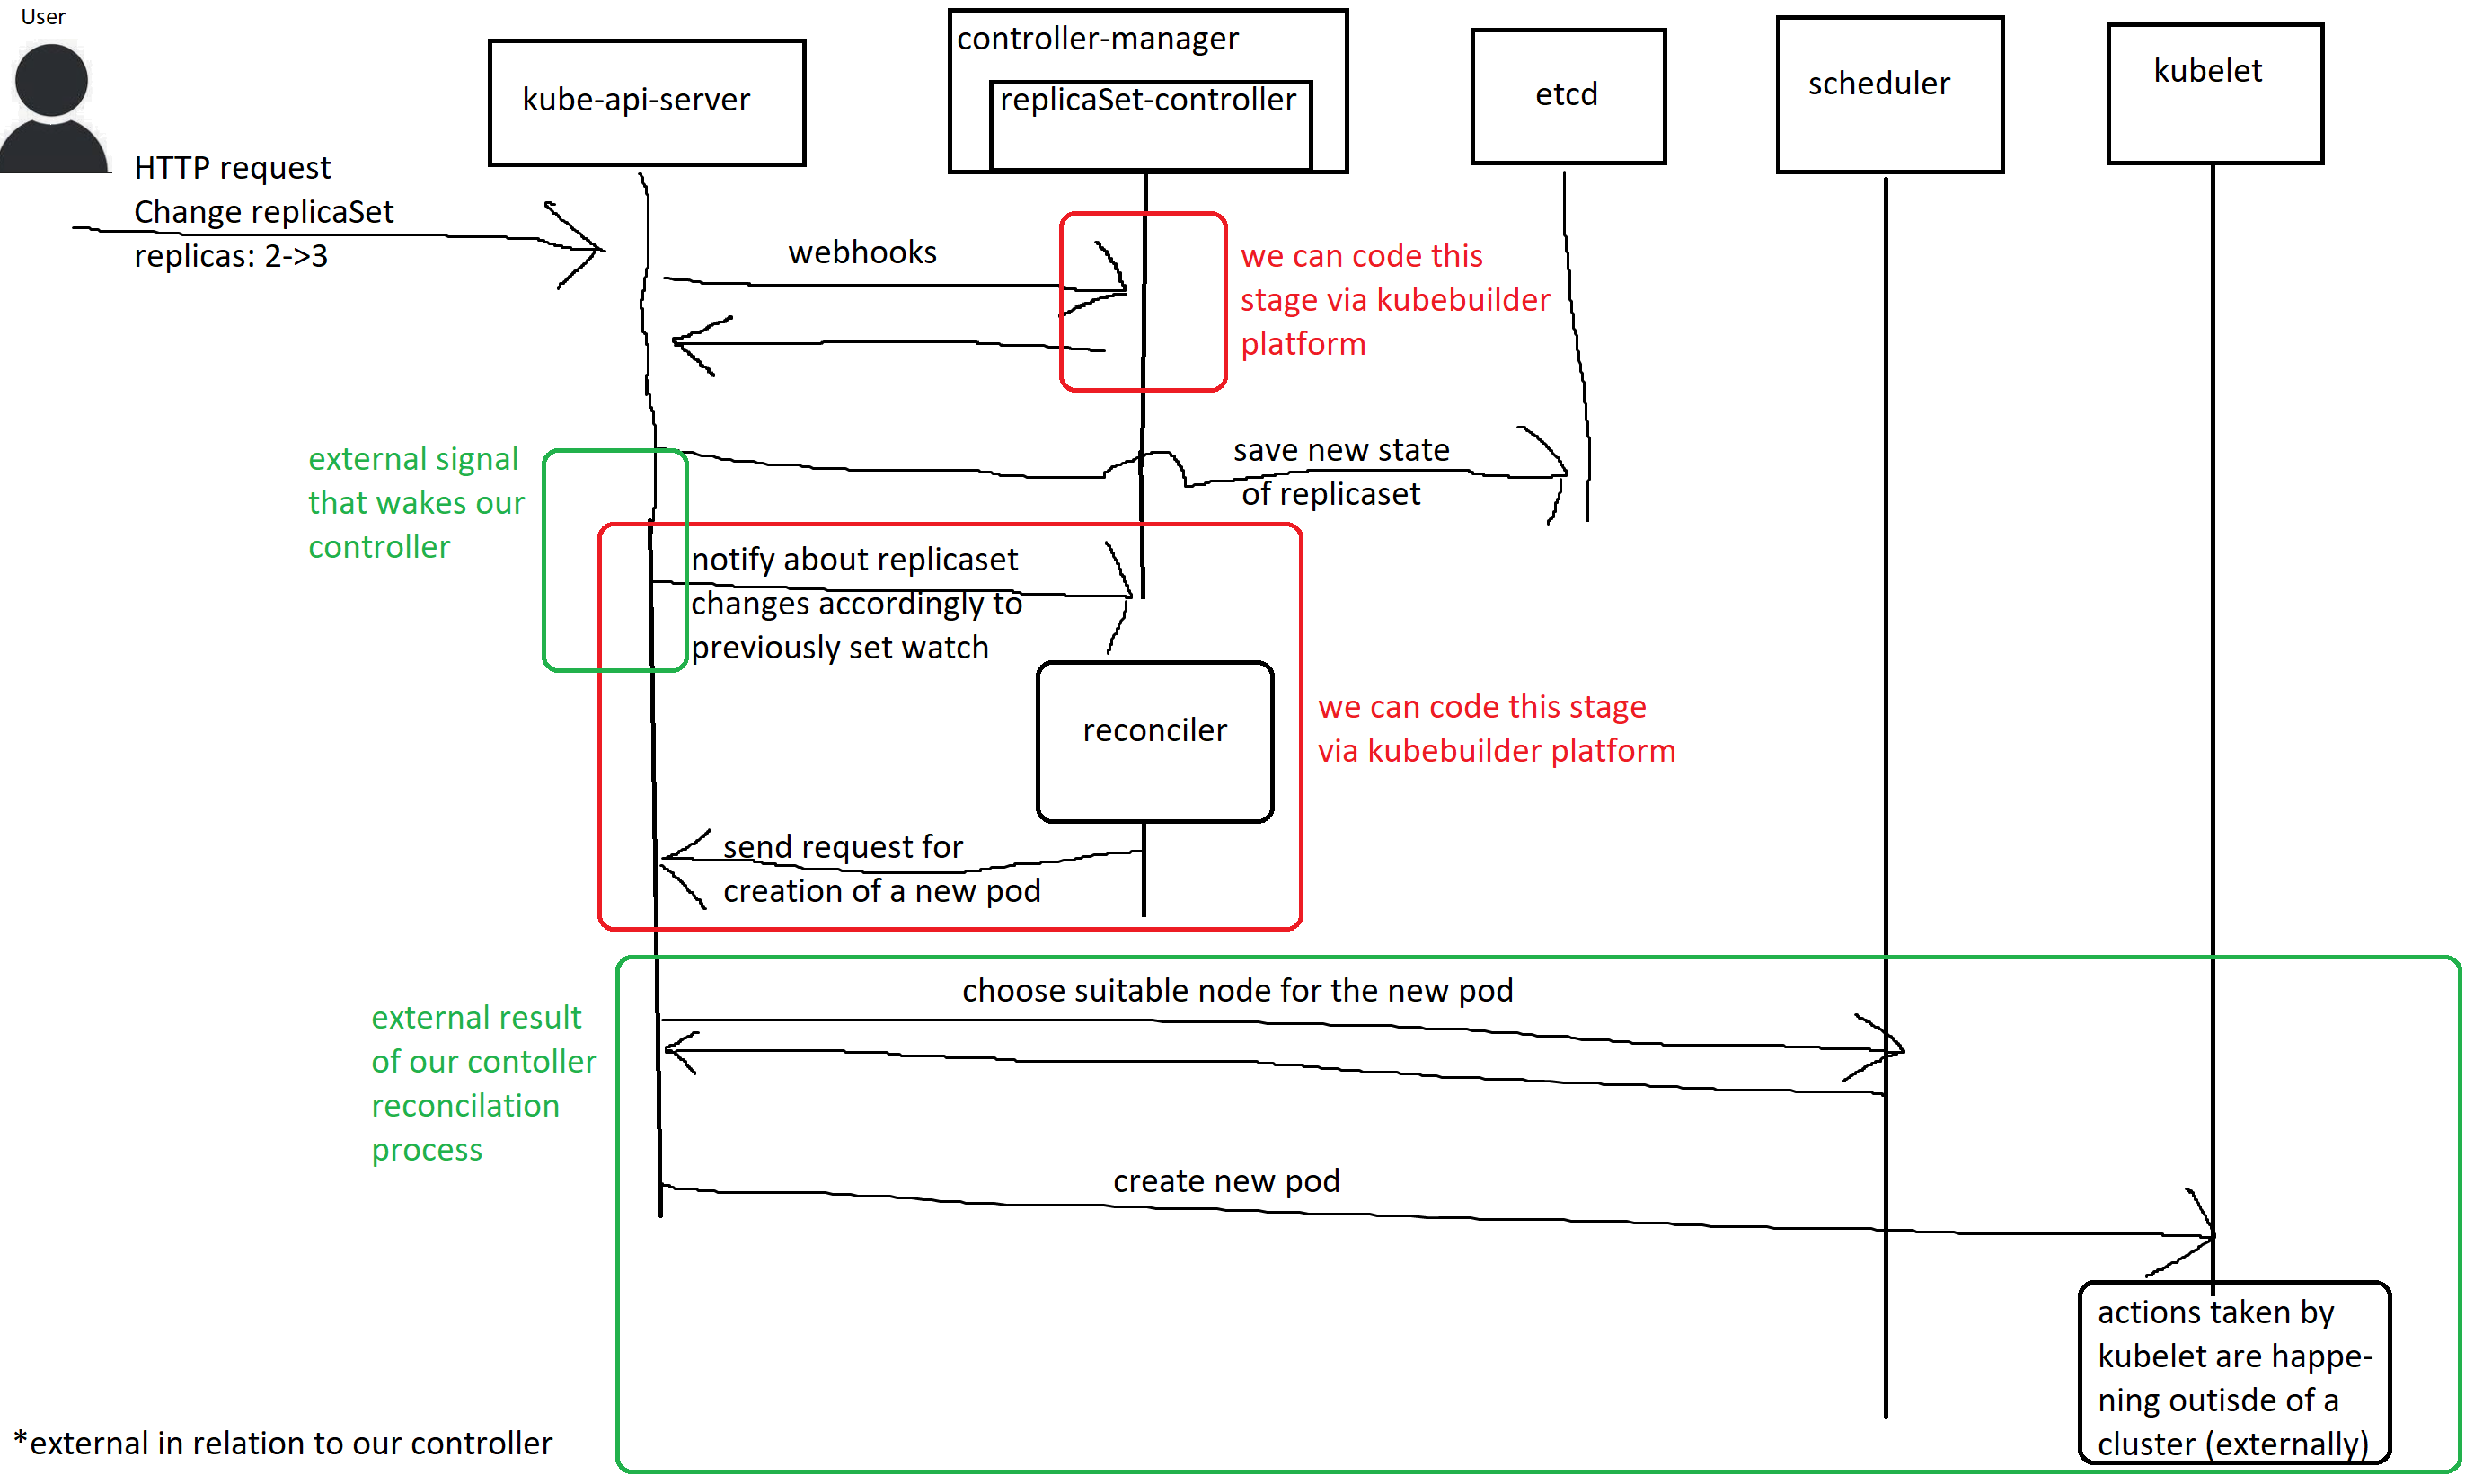
\includegraphics[width=1\linewidth]{42-flow2.png}
    \caption{Zaznaczenie możliwych do zaprogramowania elementów flow pracy kontrolera. Źródło: Opracowanie własne.}\label{fig:42-flow2}
\end{figure}